\chapter{Application Implementation}
This chapter shows some interesting parts of the implementation of the application.

\section{Subterm}
The subterm datatype is at the heart of the application.
It is probably the most important datatype,
as it is used all across the application.

\subsection{Strengths of the Subterm Datatype}
The subterm datatype has been designed to always contain a valid subterm.
An alternative to the subterm datatype would have been to simply use a term in combination with the position.
If the term and position aren't managed together though and it would be possible to change them independently,
it would be possible to create term/position combinations that are not valid.

One can take a binary tree as an example that is supposed to keep track of mathematical operations.
For example the expression \texttt{1 + 2}.
The whole term would have position \texttt{[]}, the number 1 would have position \texttt{[0]} and the number 2 would have position \texttt{[1]}.
If one were to evaluate the term independently from the positions,
One would be left with the term \texttt{3}, where only the position \texttt{[]} is valid.
However, one might still have access to the subterms at position \texttt{[0]} and \texttt{[1]}.
This would pose a problem,
as they are not valid positions anymore.
If one were to use one of the invalid positions it could cause errors.
To prevent these errors,
one might be tempted to wrap the whole thing into the Maybe Monad or use checks before using these subterms.
This would complicate things and would definitely not be a nice or elegant solution.

A more elegant solution is to wrap the term and position in a datatype,
the Subterm datatype in this case.
By not letting other Modules access the constructor of the Subterm datatype,
independent mutation of the term or position can be prevented.

A Subterm datatype can only be created using certain functions defined in the TermClass module.
This ensures that all Subterms are valid.
Thus, they can be used without having to worry about any errors arising.

\ \\
Through the many functions that are defined in the TermClass module,
reduction rules can be defined easily using f.ex. the replace function.
It takes only two simple functions in order to be able to implement the Subterm datatype.
This makes the Subterm datatype very versatile and universally usable.

\subsection{Weaknesses of the Subetrm Datatype}
Though the Subterm datatype has many strengths and is generally a very elegant implementation of the subterm concept,
it also comes with a couple of drawbacks.
These drawbacks are fairly minor though and could be patched during future development.

\ \\
The first thing that is a bit inconvenient is that every term structure implementing the Term class has to also implement the Highlightable class,
if stepping capabilities are desired.
For this purpose,
each underlying term structure needs to implement annotations or another concept to be able to store the information needed to highlight/style the terms.

This could be avoided if the Subterm datatype would support annotations out of the box.
It might be possible to find a solution,
where a dictionary containing the position as key and the annotation(s) as value could be added to a term implementing the Term class.
This might add a bit of extra effort that is needed to manage the annotations,
but on the other hand, it would come with many benefits.
Another approach using the Term class could also be possible,
like for example adding a function that determines whether a given subterm is an annotation and skipping all annotations somehow when determining the position of another subterm.

As already mentioned, the annotations - and thus the highlighting - would only need to be implemented once.
This would reduce the effort that is needed to add additional languages that could be stepped,
as the implementation is already there for any datatype implementing the Term class.

It is also important to note that the implementation of the annotations as it is now is not trivial.
Something that needs to be made sure of is that adding an annotation does not mess with the position of a term.
If the annotation is added in the middle of the term somewhere,
it is possible that it moves the positions of all subterms that come after the annotation.
Taking the previous example again and adding a random annotation shows the problem:
Going from \texttt{1 + 3} to \texttt{1 + some\_annotation(3)} can move the position of the number \texttt{3}.
While the other positions stay the same, the position of the number \texttt{3} now changes from \texttt{[1]} to \texttt{[1,0]},
while the position of the annotation now would be \texttt{[1]}.

This can cause problems when trying to combine annotations for the same term.
A single Subterm value can only point to one single subterm in the term because of how the Subterm datatype is implemented.
But often, multiple subterms in the same term need to be highlighted.
For example, the diff and the selection in the manual and interactive modes need to be highlighted in the same term.
To be able to do that the annotations need to be combined.
If one of the annotations changes the position of the actual subterm,
the other annotation might be referring to a subterm that does not exist, which could cause errors.
This problem is shown in \ref*{fig:highlightMismatch}, where the same term is annotated in two different ways and the annotations contain conflicting positions for the same subterm.

\begin{figure}[!ht]
    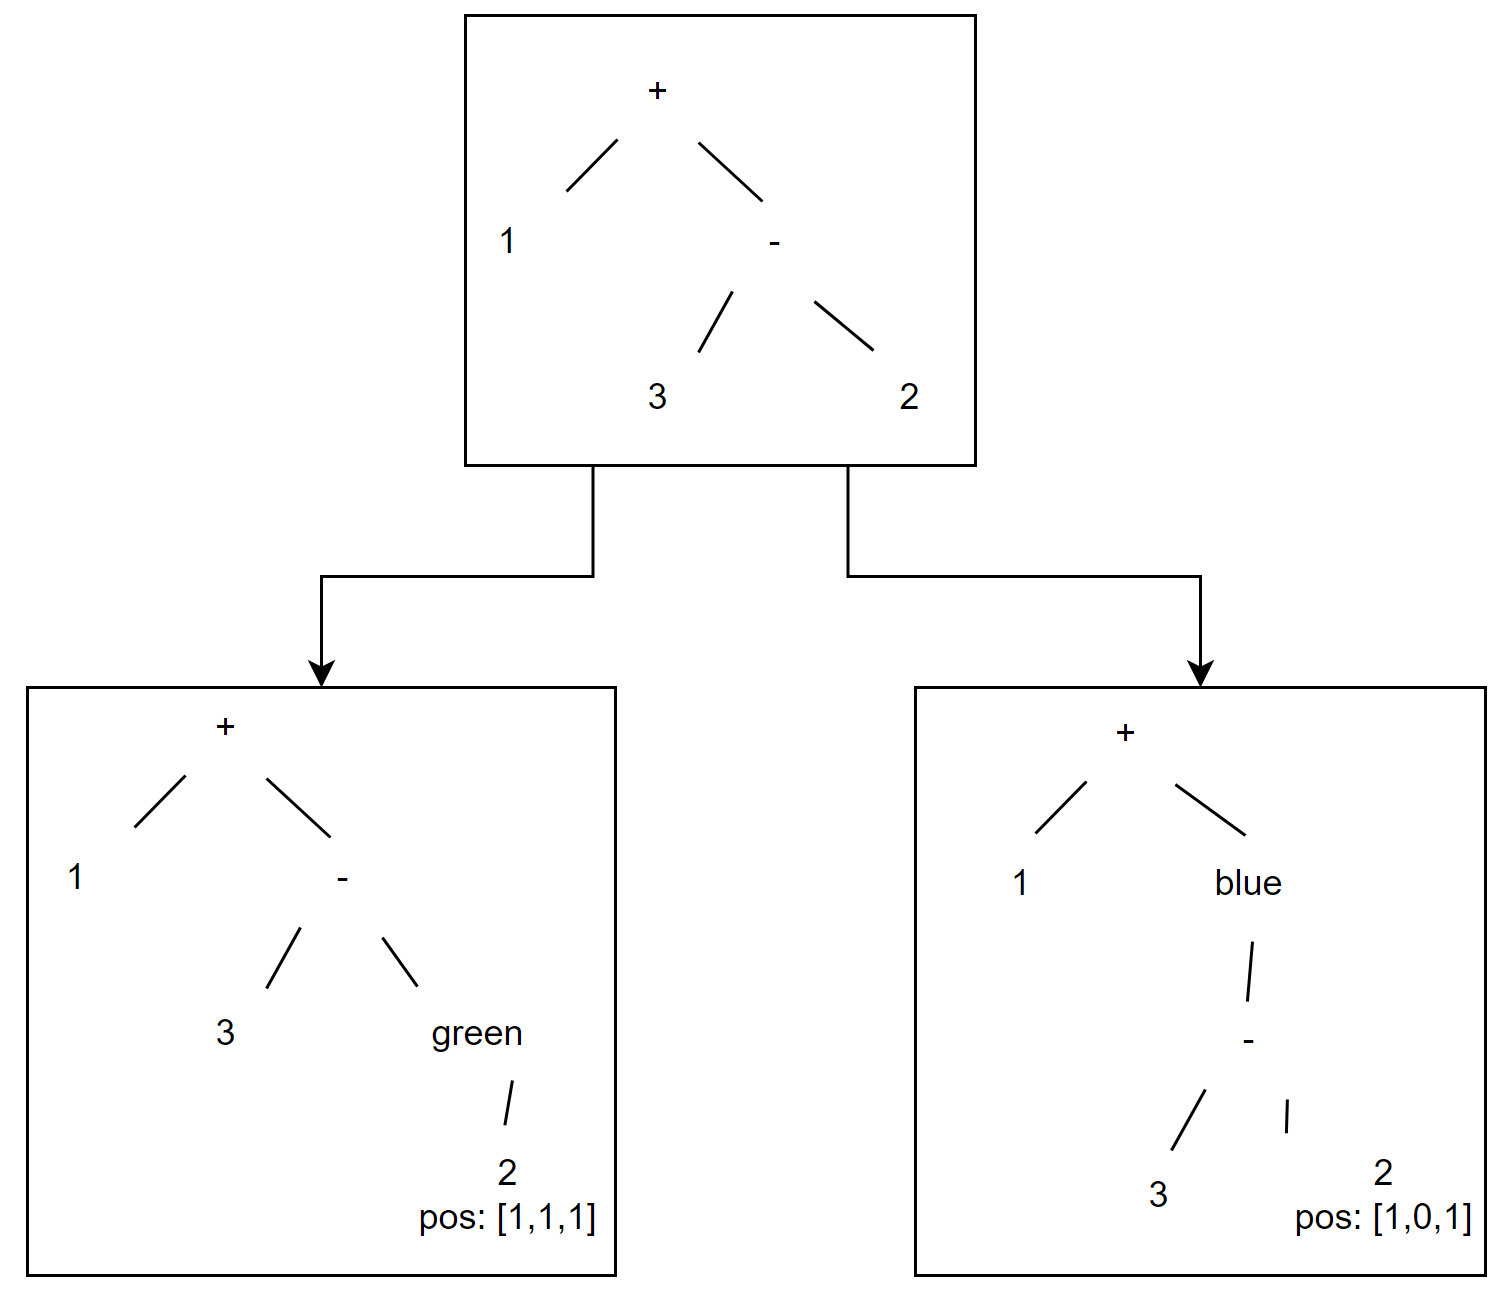
\includegraphics[width=0.75\textwidth]{resources/highlighting_mismatch.png}
    \caption{The same term can be annotated in two conflicting ways. On the left side, the position of the number 2 is [1,1,1] while on the right side, it is [1,0,1] and the position [1,1] does not exist at all.}
    \label{fig:highlightMismatch}
\end{figure}

For this reason, the annotations must not change the positions of any subterm in the term.
Implementing a solution that does not do that might not be obvious initially.

In the Core implementation of the Term class, this is handled by making the annotation appear to be the last child of its parent term,
while the children of the annotation appear to be children of the annotation's parent as well.
This preserves the position of the annotation's children, while still making the Term class aware of the annotation's existence.

The impact that this change has is shown in \ref*{fig:highlightMismatchResolved}.
It is important to note that it might look like with this implementation one cannot tell which child the annotation refers to,
but this is only a problem when looking at the subterm in this form.
Internally in the Core representation, it is still well-defined which child the annotation refers to.

\begin{figure}[!ht]
    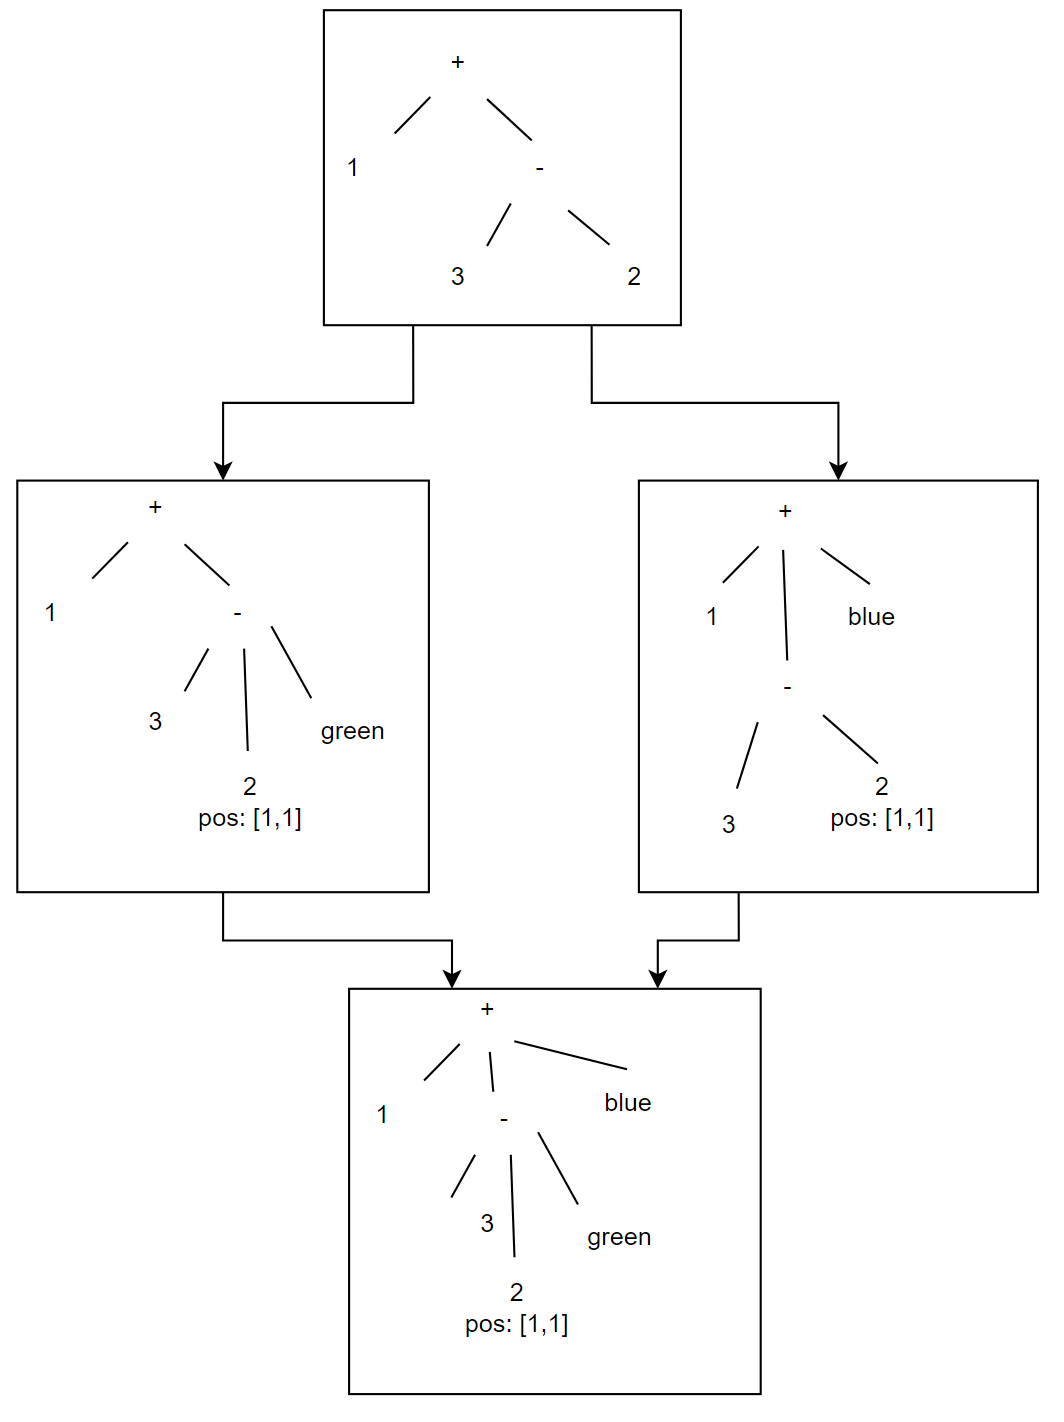
\includegraphics[width=0.75\textwidth]{resources/highlighting_mismatch_resolved.png}
    \caption{The same term, again annotated in two different ways, this time however they are not conflicting and can be combined.}
    \label{fig:highlightMismatchResolved}
\end{figure}

\ \\
The second thing that is also a bit inconvenient is that a Subterm value can only point to one subterm in the term.
Especially for beta reductions,
it would be convenient if one could for example select multiple subterms with a filter condition.

As it is right now,
to fully beta-reduce a term,
the subterms need to be replaced individually.
When attempting a beta reduction,
all subterms matching the binding variable are gathered from the term.
This yields a list of subterms as a result.
To replace all occurrences,
the first subterm is selected and the beta reduction is performed on that subterm.
The other subterms are left untouched.
Then, on the replaced subterm,
all subterms matching the binding variable are gathered again and the process is repeated until the binding variable does not occur anymore.
This is somewhat cumbersome,
but there is no way of replacing multiple subterms in a single term due to the implementation of the Subterm datatype.

A solution for this problem could be, as mentioned before,
the capability to select all subterms meeting a certain criterion inside of the subterm and replace them all in one go.
This approach could be implemented more efficiently than the current approach.


\section{Derivation}
The Derivation datatype is responsible for keeping track of the history of the derivation.

\subsection{Initial Approach}
Originally,
it was planned to be a tree data structure,
but it was dropped in favor of a list for simplicity and because making it a tree did not have any benefits.
One of the first versions of the Term and Derivation datatypes can be seen in \ref*{fig:originalDerivation}.

\begin{figure}[!ht]
    \begin{verbatim}
    data Term
        = Redex String [Term] (Maybe Term)
        | Value String deriving Show
    
    data Derivation = Term [(Derivation, RewriteRule)]
    \end{verbatim}
    \caption{One of the first drafts for the Derivation Type}
    \label{fig:originalDerivation}
\end{figure}

The Term datatype turned out to not work well at all and was thus discarded quickly.
The Derivation data type on the other hand was considered for a longer time.
The idea was to keep track of every possible way to derive a term.
So once a branch of the tree was discovered through stepping,
the information would be saved even if the user decided to step back.
If the user would go back down the same path at a later point,
the information would be available already and no computation would be necessary.

The plan was to count all redexes in the current term
and to create an entry in the list for each of the redexes,
thus creating a tree.
And as soon as one of the redexes was selected by the user,
the respective entry in the list would be adjusted.

In the end, however,
a simpler approach was taken,
as the overhead for re-calculating a step is not that big and thus the original datatype did not offer too much of a benefit.
In addition to that,
the tree datatype would grow exponentially if all paths were discovered and would unnecessarily take up space.

Another reason why it was dropped is that it did not seem like a very likely use case,
as a user would probably mostly be interested in just stepping one path and not all of them.

\subsection{Final Version}

The final version of the Derivation datatype is a lot simpler than the original tree structure.
It is in essence a stack data structure that only keeps track of the current history and discards the current term if the user decides to step back.
Since the current history is most likely the only thing the user cares about,
removing all other branches seemed to make a lot of sense.
The final version of the Derivation datatype can be seen in \ref*{fig:finalDerivation}

\begin{figure}[!ht]
    \begin{verbatim}
    data Derivation t where
        Derive :: Reducible t => t -> [DerivationStep t] -> Derivation t
    
    type DerivationStep t = (RewriteRule t, RuleDescription, Subterm t)
    \end{verbatim}
    \caption{The final and current version of the Derivation datatype.}
    \label{fig:finalDerivation}
\end{figure}

The Derivation datatype consists of the original term,
which is the first argument to the constructor,
and a list of derivation steps,
which is the second argument.
The reason the starting term is stored separately from the other derivation steps
is that it does not require the additional information that the DerivationStep datatype provides,
like RewriteRules or RuleDescriptions.
Also,
the starting term should not specify a certain subterm,
which is why it is just of type t and not Subterm t.

\subsection{DerivationStep}
The DerivationStep datatype is closely linked with the Derivation datatype.
It is used to specify the rule that has been applied,
a description of the rule that has been used,
and the resulting term.

The RuleDescription is currently just a simple datatype as it does not contain a lot of information.
It is used to display the justifications for the steps.
The RuleDescription datatype could be expanded to contain more (meta)information,
like line numbers of the function definition, etc.
but this was not necessary yet, nor was there a concrete use case for this.

The resulting term is of type Subterm t
and the subterm that is pointed to
is the subterm that has been substituted when applying the rule.
This allows for easy highlighting of the diff.
All that needs to be done is to annotate that Subterm with the style for diffs.
When the term is printed, the diff will show up via annotation.

\section{RewriteRule}
The RewriteRule datatype is used to create rules for the derivation at runtime.
While most rules are defined at compile time already,
like beta reductions and case applications which always follow one specific pattern,
some rules cannot be determined at compile time.
The most important examples of RewriteRules are delta reductions.
To create these RewriteRules for delta reductions,
the top-level bindings from the module are collected and turned into RewriteRules.

A RewriteRule is just a function that takes a Subterm and returns a Maybe,
which might contain the term that results from the application of the rule.
The definition of RewriteRule can be seen in \ref*{fig:RewriteRule}

\begin{figure}[!ht]
    \begin{verbatim}
    type RewriteRule t = (Subterm t -> Maybe (t, RuleDescription))
    \end{verbatim}
    \caption{The RewriteRule datatype.}
    \label{fig:RewriteRule}
\end{figure}

To create a rule for a specific delta reduction,
the Substitution Stepper goes through all top-level bindings and creates RewriteRules.
If the subterm that the rule is applied to matches the identifier of the binding,
the definition of the binding is returned,
otherwise, Nothing is returned.
This makes sure that the rule for a delta reduction can only be applied to matching identifiers.

Another example of a RewriteRule is a Let binding,
which are treated as delta reductions that can only be applied to children of the Let binding.

\section{Reducible}
The Reducible class is the main class when it comes to the stepping of terms.
It provides an interface that allows the Substitution Stepper to derive any term that implements this class.
To implement the class, two functions are needed.

\subsection{\texttt{reduce}}
The \texttt{reduce} function is used to derive one step of a term.
It takes a set of RewriteRules and a Subterm and tries to derive the specified subterm.
If a reduction can be applied to the subterm,
the resulting term and RuleDescription are returned, otherwise, Nothing is returned.

In the case of Core,
the \texttt{reduce} function first tries to do a case application,
then a beta reduction,
then a delta reduction,
then resolving a Let binding,
and lastly applying a Let binding to a variable.
If none of these work,
Nothing is returned,
otherwise, the first type of reduction that yields a result is returned.

\subsection{\texttt{isWHNF}}
The second function required to implement the Reducible class is \texttt{isWHNF}.
This function is needed to implement two different types of derivation strategies.

The first type of strategy strictly follows the ordering defined by the strategy.
The second type of strategy follows the ordering partially.
First, all terms that are not contained within a term that is in WHNF are looked at and the strategy is applied to only these terms.
If, however, there are no reducible terms outside of terms that are in WHNF,
the terms contained in these WHNF terms are considered too.

This is supposed to prevent infinite loops that could arise when using the leftmost innermost strategy.
An example of this is the lambda \texttt{\\x y -> x + y} with the definiton of \texttt{+} being \texttt{0 + x = x; (y + 1) + x = y + (x + 1)}.

If the leftmost innermost strategy is followed strictly,
the definition of \texttt{plus} will be expanded infinitely, resulting in infinite recursion,
because the \texttt{+} operation is nested more deeply than the application of the lambda.

If, however, terms inside of terms that are in WHNF are not considered,
then the definition of \texttt{+} could not be expanded any further.
This is because the lambda is in WHNF,
thus the lambda needs to be applied to the arguments first before the definition of the \texttt{+} can be expanded.

This limitation still does not prevent all infinite loops though.
If a term does not have a normal form,
this approach will not terminate.

\subsection{Strategies}
The ReducibleClass also contains the derivation strategies that can be used by the Substitution Stepper to step through terms.
However, in retrospect,
this approach does not work well since the derivation strategy cannot be generalized for any given type of term.
The strategies that are currently defined order the subterms according to their numbering if the term is traversed infix.
This, unfortunately, does not work for Core as it is not infix.

Despite this flaw, the leftmost outermost and call-by-name strategies work reliably for Core.

\section{Normalizable}
The Normalizable class is an extension of the Reducible class.
Its use case is to be able to find a sequence of 'atomic' steps,
in order to be able to skip the uninteresting parts of a derivation.

Taking Core as an example,
in the case of a delta reduction,
the Normalizable implementation counts the number of lambdas nested in the function definition,
and then tries to find the same amount of applications surrounding the lambda,
thus allowing to do delta- and beta reductions, as well as case applications in one single step, hiding the details.

This hides the details of the stepping that most users probably would not want to see either way.


\section{Highlightable}
The Highlightable class is responsible for annotating terms with styles,
so that the terms can then be highlighted during pretty printing.

As discussed in the section about Subterms,
it might have been more advantageous to leave the annotating to the Subterms.
With the current implementation,
the Highlightable class has 4 functions that need to be implemented.

\subsection{\texttt{annotateTerm}}
The function annotateTerm is responsible for annotating Subterms with styles.
In the implementation for Core,
source note Ticks are used to add styles to the Expr datatype.

Since the styles implement Show and Read,
they can easily be added as source notes and then transformed back into actual styles.

\subsection{\texttt{combineAnnotations}}
The function combineAnnotations is used to combine the annotations of two subterms of the same root term.
This needs to be done due to the previously mentioned limitation that it is not possible to annotate two different subterms in the same Subterm datatype.

As a workaround,
the combineAnnotations function checks whether the root terms of the Subterm datatypes are equal,
and if that is the case the annotations contained in the two root terms are combined.
This allows the Substitution Stepper to annotate both the selection and the diff in the same term.

\subsection{\texttt{highlight}}
The highlight function takes a (potentially) annotated term and pretty-prints it.
The reason that this function is needed,
is that the regular pretty function does not support colors or any other form of highlighting.
As the signature of the pretty function is \texttt{pretty :: t -> Doc ann},
the highlight function, however, wants to have the signature \texttt{highlight :: t -> Doc AnsiStyle}.

The AnsiStyle annotation provides the coloring/underlining functionality that is used by the Substitution Stepper.
So the highlight function needs to call a function different from pretty,
that supports these AnsiStyle annotations.

To prevent code duplication,
in the case of Core,
a function called prettyEx is defined that produces results of type Doc AnsiStyle.
The highlight function can then just call the prettyEx function,
while the pretty function calls \texttt{unAnnotate . prettyEx},
turning the \texttt{Doc AnsiStyle} result back to a \texttt{Doc ann} result.

This way the pretty printing logic only needs to be implemented once.

\subsection{\texttt{unAnnotateTerm}}
The function unAnnotateTerm removes all annotations for a certain term,
as the name suggests.

\section{User Interaction}
The user interaction was mainly done using the Haskeline package for writing and reading output/input
and the System.Console.ANSI package to manipulate the CLI so that the output looks presentable and not overloaded.

\subsection{Haskeline CompletionFunc}
The Haskeline CompletionFunc is usually used to complete file paths and words via the tab key while inputting on the CLI.
The Substitution Stepper uses the CompletionFuncs a bit differently though.
Instead of completing any input,
the tab key cycles through the available redexes.

The detour via the CompletionFuncs was taken because there is no other easy way to get tab key or arrow key input from the CLI.
And since using the tab key is much more convenient and intuitive compared to typing in a command or something,
this approach was selected.

A drawback here is that there is no easy key to cycle the redexes in reverse order,
as Haskeline only supports the tab key for the completion of words.
For reverse-cycling of the redexes the 'backTab' command can be typed in.

\subsection{Removal of Old Prompts}
To remove clutter on the UI,
some commands remove the previous prompt before printing the new one.

A very good example of this is the tab command,
which changes the selected redex.

Normally,
the same term would be printed out under the previous one,
with the only difference being the coloring of the selected subterm.
Since this can clutter up the UI when changing the selection a lot,
the functionality to remove the previous prompt was introduced.

Due to this it now looks like the green-colored selection jumps around in the same term,
giving the illusion of a UI that can update itself.
In the background,
a certain amount of lines are deleted on the CLI and re-printed with a different coloring.

The same approach was also chosen when a command is entered,
that is not valid or when error messages are printed.
This avoids the constant moving of the CLI when there are no changes in the term itself.

\subsection{Printing under the Cursor}
Some commands that can be used when deriving manually produce output.
This output can be either an error message or just a regular 'success' message,
that conveys information to the user.
To keep the history of terms above the cursor stable and uninfluenced by these messages,
the messages are printed under the cursor.

This also greatly simplifies the erasing of the messages.
While the prompts can be easily erased, even if they are above the cursor, since their length is known to the application,
the length of the messages is not known.
Thus there is no easy way to delete them if they are written above the cursor.

If they are written below the cursor, however,
the application can simply clear the CLI until the end of the screen is reached.
A solution to this is discussed in section \ref*{subsect:UIState}.
Unfortunately, there was not enough time to implement the suggested changes properly.

\ \\
To be able to print under the cursor,
the message-outputting functions print a newline,
moving the cursor down one line.

Before the message is printed,
the number of lines that the message will occupy is calculated.
Then the message is then printed.
After this,
the cursor is moved back up to where it was originally.
This gives the illusion of messages being printed under the cursor.

From the number of lines occupied by the message,
the application can calculate how many lines the cursor needs to be moved up.

\subsection{Adaptive Line Width}
To be able to take advantage of the full terminal,
the UIUtils module provides a function that creates a LayoutOpts value,
which is used by the pretty printer.

The LayoutOpts value contains the length of a line in the CLI.
This allows the pretty printer to format the terms and messages in a way that
allows them to fill up the entire screen.
Line breaks are chosen smartly by the prettyprinter,
so that words should not spill over to the next line,
avoiding ugly line breaks.

The function used to get the width of the CLI is not guaranteed to work on any terminal,
as it is not part of the ANSI standard functionality.

In case the width of the CLI cannot be retrieved,
80 characters per line is chosen as the default value,
as most terminals should be at least this width.

\section{Commands}
For the user interaction, the Command datatype is used.
The list of commands is easily extensible,
thus allowing for the easy addition of new commands.
The Command datatype can be seen in figure \ref*{fig:Command}

\begin{figure}[!ht]
\begin{verbatim}     
type CommandResult = Either (Doc AnsiStyle) (Maybe (Doc AnsiStyle))

data Command t = Command
    { name              :: String
    , argsDescription   :: String
    , usageDescription  :: String
    , command           :: [String] -> State (DerivationState t) CommandResult
    , continueAfter     :: Bool
    , replaceLine       :: Bool
    , printDerivation   :: Bool
    }
\end{verbatim}
    \caption{The Command datatype.}
    \label{fig:Command}
\end{figure}

Each command has access to the DerivationState and can thus modify the derivation freely.
Commands cannot perform IO actions,
but they can notify the user about errors and pass messages via the CommandResult.

If the CommandResult is \texttt{Left someDoc},
it means that an error has occurred and the message is displayed in red.
If an error occurs,
the DerivationState should not be changed.

If the CommandResult is \texttt{Right maybeDoc},
then the command was successful and depending on the content of \texttt{maybeDoc} there can be a message that should be conveyed to the user.

\ \\
While the Commands can also not read input via IO actions,
the user can pass arguments to the Command via a list of strings.
It is the Command's responsibility to parse/read the arguments correctly and without producing an error that terminates the application.

\ \\
The user is able to call commands by typing in their names,
followed by a space-delimited list of arguments if needed.

\ \\
The remaining fields in the Command datatype give the Command control over what happens after the command is executed.

For example, the continueAfter flag will decide if the derivation continues after the command is executed.
If it is set to False, the derivation will stop.
This is used for the quit command, which simply aborts the derivation.

The replaceLine flag decides whether the previous prompt should be removed before the new one is printed,
as described in the previous section about the UI.
The tab command is one of the examples that make use of that flag.

The printDerivation flag decides whether the derivation should be printed out.
The flag only takes effect if the derivation stops after the command is executed.
An example of a Command that uses this flag is the continue command.
Since the command continues derivation automatically,
the user cannot see what is happening,
thus it needs to be printed at the end so the user can see it.

\ \\
All the current commands can be executed using a combination of these flags,
however, if new commands are added the list of flags might have to be extended.

\ \\
The reasoning behind implementing user interaction this way,
is, as mentioned before, to be able to easily add new commands.
The inspiration for this was taken from the Command software design pattern.
